\documentclass{beamer}

\usetheme{default}
\usecolortheme{dove}
\AtBeginSection[]
{
  \begin{frame}
    \centering
    \Huge \insertsectionhead
  \end{frame}
}

\setbeamertemplate{footline}[page number]
\beamertemplatenavigationsymbolsempty

\usepackage{booktabs}
\usepackage{multirow}
\usepackage{import}

\usepackage[backend=biber,style=authoryear,
	maxcitenames=1,uniquelist=false,uniquename=false]{biblatex}
\addbibresource{references.bib}

\title{Work summary}
\subtitle{Summary of all the existing materials that are relevant for the
2\textsuperscript{nd} paper}
\author{Kamal Ahmadov}
\institute{University of Strasbourg}
\date{\today}

\begin{document}

\frame{\titlepage}

\begin{frame}
	\begin{itemize}
		\item ramp injection rate
		\item radial diffusion
		\item summary table of scaling
		\item velocity-duration
		\item seismicity rate
	\end{itemize}
\end{frame}

\begin{frame}
	\frametitle{Quasi-linear seismic front migration is not explained by a
		nonlinear diffusion process}

	\begin{columns}
		\begin{column}{0.4\textwidth}
			\begin{itemize}
				\item Scaling exponents vary across sites
				\item Linear seismic migration is only explained by aseismic slip
				\item Effect of deformable fracture on seismic migration is less studied
			\end{itemize}
		\end{column}
		\begin{column}{0.6\textwidth}
			\resizebox{\textwidth}{!}{
				\begin{tabular}{llll}
					\toprule
					Site & Source                   & $\alpha$ & Mechanism              \\
					\midrule

					\multirow{5}{*}{Soultz 1993}
					     & \cite{ShapiroEtAl2002}   & 0.5      & Linear diffusion       \\
					     & \cite{GoebelBrodsky2018} & 0.5      & -                      \\
					     & \cite{DeBarrosEtAl2021}  & 0.65     & Aseismic slip          \\
					     & \cite{SaezUribe2023}     & 1        & Aseismic slip          \\
					     & \cite{DanreEtAl2024}     & 1        & Aseismic slip          \\
					\midrule

					\multirow{4}{*}{Basel 2006}
					     & \cite{JohannEtAl2016}    & 0.49     & -                      \\
					     & \cite{GoebelBrodsky2018} & 1        & -                      \\
					     & \cite{DeBarrosEtAl2021}  & 0.7      & Aseismic slip          \\
					     & \cite{DanreEtAl2024}     & 1        & Aseismic slip          \\
					\midrule

					\multirow{3}{*}{Cooper}
					     & \cite{GoebelBrodsky2018} & 0.5      & -                      \\
					     & \cite{JohannEtAl2016}    & 0.28     & Nonlinear diffusion    \\
					     & \cite{DeBarrosEtAl2021}  & 0.5      & -                      \\
					\midrule

					\multirow{3}{*}{Fenton Hill 1983}
					     & \cite{ShapiroEtAl2002}   & 0.5      & Linear diffusion       \\
					     & \cite{HummelMller2009}   & 0.5      & Nonlinear diffusion    \\
					     & \cite{GoebelBrodsky2018} & 0.5      & -                      \\
					\midrule

					Rittershoffen 2013
					     & \cite{LenglineEtAl2017}  & 1        & Aseismic slip          \\
					Rittershoffen 2016--2024
					     & \cite{LenglineEtAl2025}  & 0.5      & -                      \\
					\midrule

					KTB 1997
					     & \cite{ShapiroEtAl1997}   & 0.5      & Linear diffusion       \\
					Barnett Shale
					     & \cite{ShapiroDinske2009} & 1/3      & Nonlinear diffusion    \\
					LSBB, France
					     & \cite{DuboeufEtAl2017}   & 0$^{1}$  & Aseismic slip          \\
					St. Gallen
					     & \cite{GoebelBrodsky2018} & 1        & -                      \\
					Paralana, Australia
					     & \cite{GoebelBrodsky2018} & 1        & -                      \\
					Landau
					     & \cite{GoebelBrodsky2018} & 0        & -                      \\
					Paradox, Colorado
					     & \cite{GoebelBrodsky2018} & 1        & -                      \\
					Oklahoma, USA
					     & \cite{GoebelEtAl2017}    & 0        & Poroelasticity         \\
					\midrule

					\multicolumn{4}{l}{$^{1}$ Seismic front lacks temporal dependence.} \\
					\bottomrule
				\end{tabular}
			}
		\end{column}
	\end{columns}
\end{frame}

\begin{frame}
	\frametitle{Modeling fluid injection into a deformable fracture}

	\begin{columns}
		\begin{column}{0.5\textwidth}
			\begin{itemize}
				\item 3DEC simulations
				\item Self-similarity of the diffusion equation $$a
					      \frac{\partial }{\partial x} \left(w^{3} \frac{ \partial w }{
						      \partial x }  \right)  = \frac{ \partial w }{ \partial t }
				      $$
				\item Asymptotic small and large time solutions
				\item Half-space solution for induced normal stress
				\item Study of the injection rate effect
			\end{itemize}
		\end{column}
		\begin{column}{0.5\textwidth}
			\resizebox{\textwidth}{!}{\import{figures/}{model-schematic.pdf_tex}}
		\end{column}
	\end{columns}
\end{frame}

\section{Constant pressure injection}

\begin{frame}
	\frametitle{Square-root migration of front in both soft and rigid cases}
	\centering
	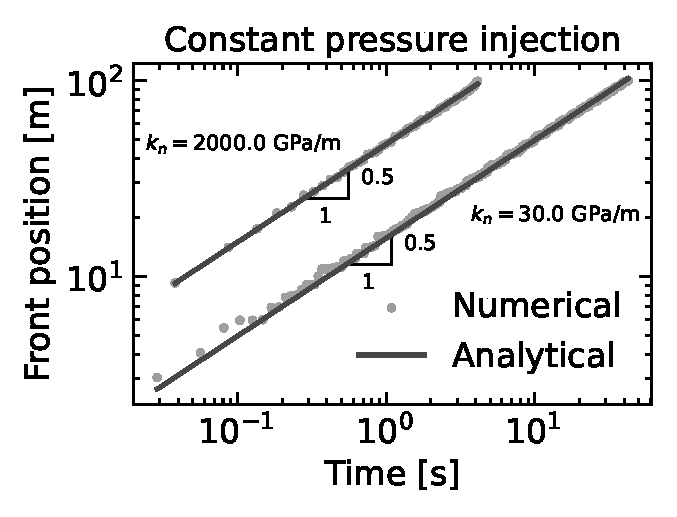
\includegraphics[width=0.8\textwidth]{figures/const-pressure-front.eps}
\end{frame}

\section{Constant injection rate}

\begin{frame}
	\frametitle{Displacement and stress boundary condition on the block produce
		similar results}

	\centering
	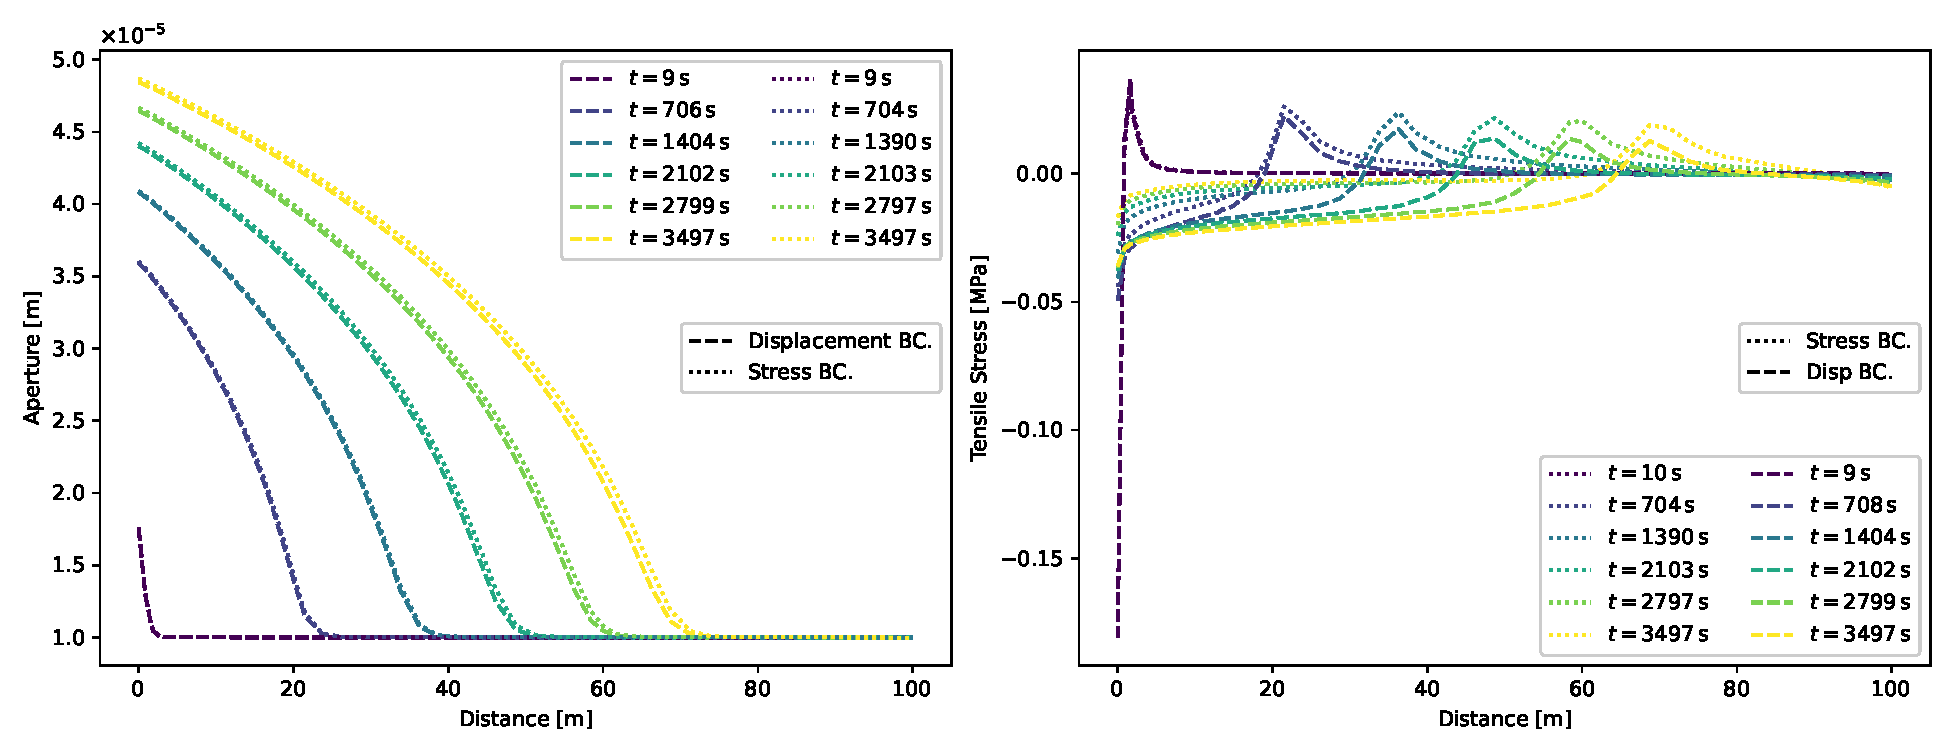
\includegraphics[width=\textwidth]{figures/effect-of-stress-bc.eps}
\end{frame}

\begin{frame}
	\frametitle{Square-root migration when $t \leq t_{c}$, quasi-linear
		migration when $t \gg t_{c}$, and a transition in between}
	There exists a characteristic time $t_{c} = \frac{k_{n}w_{i}^{5}}{12 \mu
			q_{0}^{2}}$
	\begin{itemize}
		\item When $t \leq t_{c}$, fluid flow is governed by linear diffusion (rigid)
		      $$
			      x_{f}(t) \sim a^{1/2} w_{i}^{3/2} t^{1/2}, \quad w(t) \sim
			      q_{0} a^{-1/2} w_{i}^{-3/2} t^{1/2}
		      $$
		\item When $t \gg t_{c}$, non-linear diffusion (soft)
		      $$
			      x_{f}(t) \sim a^{1/5} q_{0}^{3/5} t^{4/5}, \quad w(t) \sim
			      q_{0}^{2/5} a^{-1/5} t^{1/5}
		      $$
		\item When $t \approx t_{c}$, transition from linear to nonlinear
		      diffusion
		      $$
			      x_{f}(t) \sim t^{\alpha(t)},\ 1/2 < \alpha(t) < 4/5,
		      $$
		      $$
			      w(t)\sim t^{\beta(t)}, \ 1/2 > \beta(t) > 1/5
		      $$
	\end{itemize}
\end{frame}

\begin{frame}
	\frametitle{Numerically obtained dimensionless similarity profiles show the
		asymptotic small and large time behaviors}
	\begin{itemize}
		\item[(a)] $q_{0} = \mathsf{5 \times 10^{-9} \, m^2/s} \to t_{c} =
			      \mathsf{66667\, s} \to t < t_{c} \to \mathbf{rigid}$
		\item[(b)] $q_{0}= \mathsf{5 \times 10^{-5} \, m^2/s} \to t_{c} =
			      \mathsf{0.00067\, s} \to t \gg t_{c} \to \mathbf{soft}$
	\end{itemize}
	\vspace{8pt}
	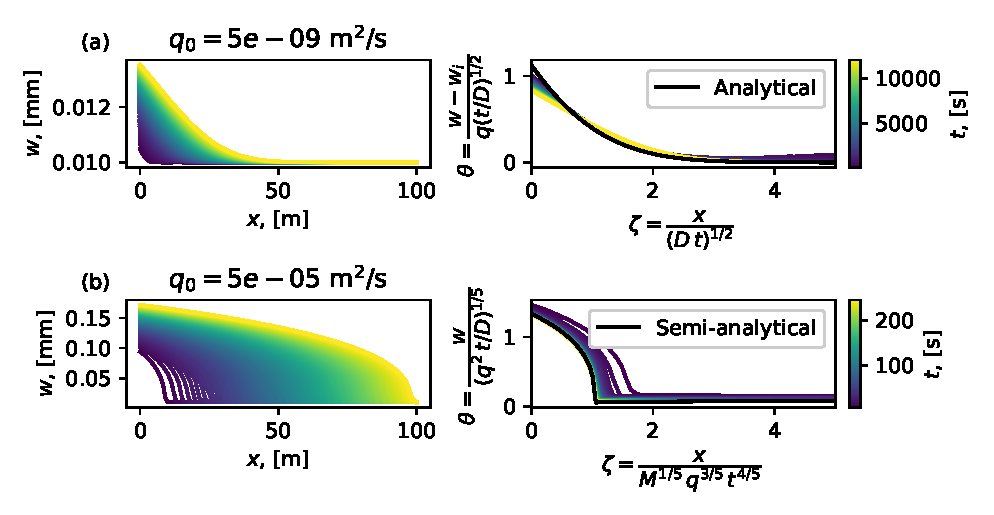
\includegraphics[width=\textwidth]{figures/similarity-profiles.eps}
\end{frame}

\begin{frame}
	\frametitle{Higher injection rate changes the scaling in time of stress
		front position and pressure at the injector}

	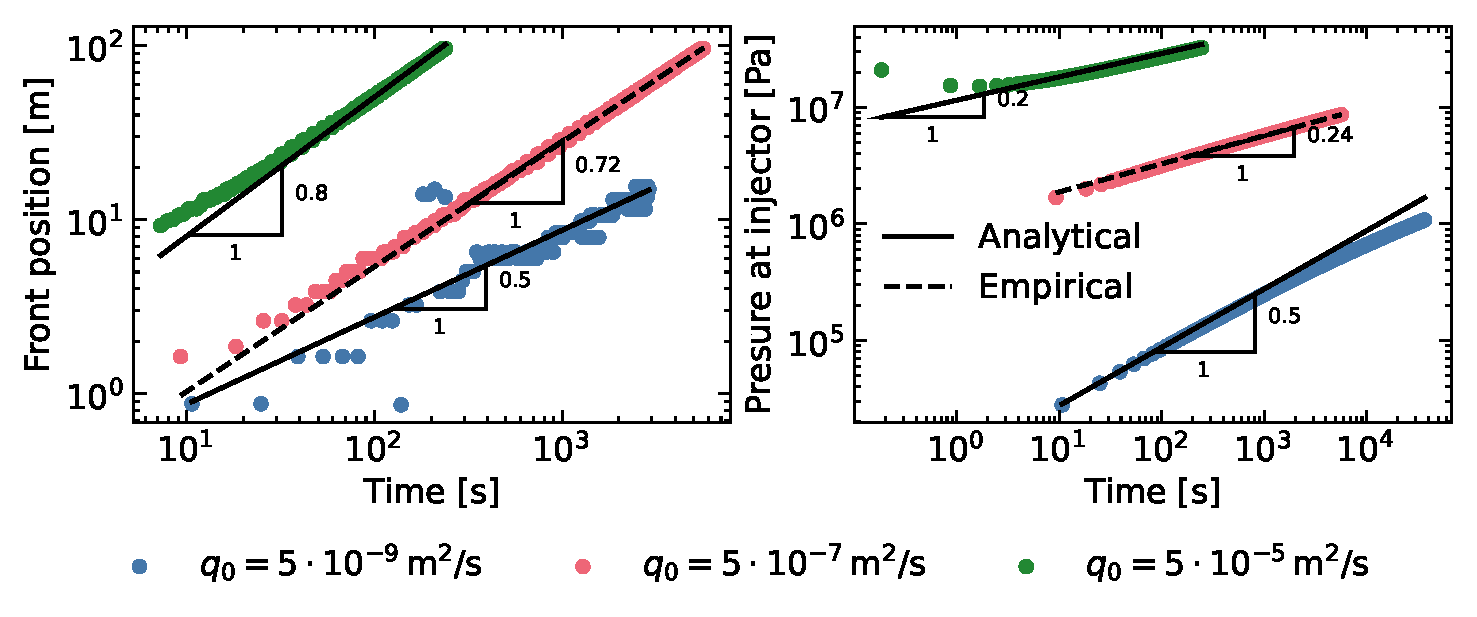
\includegraphics[width=\textwidth]{figures/front-and-p-inj.eps}
\end{frame}

\begin{frame}
	\frametitle{Dimensionless pressure at the injector evolves as rigid at
		small times, then transitions to soft}
	\centering
	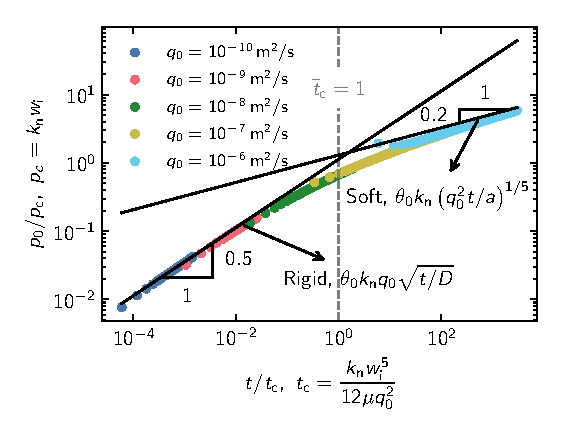
\includegraphics[width=0.9\textwidth]{figures/dimless-pressure.eps}
\end{frame}

\begin{frame}
	\frametitle{Dimensionless front follows crossover function with asymptotic
		exponents 1/2 and 4/5, and  transition scale $\delta=0.05$}
	Crossover function for dimensionless front ($t_{c}=1$):
	$$
		x_{f}(t) = \frac{A_{\mathsf{early}}t^{1/2}}{1 + (t/t_{c})^{\delta}} +
		\frac{A_{\mathsf{late}}t^{4/5}}{1 + (t_{c}/t)^{\delta}}.
	$$
	\begin{columns}
		\begin{column}{0.5\textwidth}
			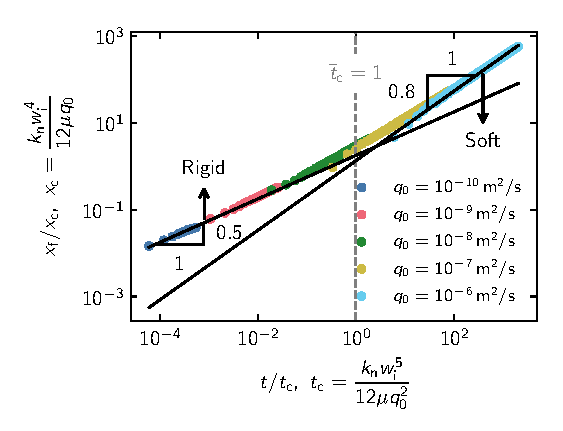
\includegraphics[width=\textwidth]{figures/dimless-front-with-analytical.eps}
		\end{column}
		\begin{column}{0.5\textwidth}
			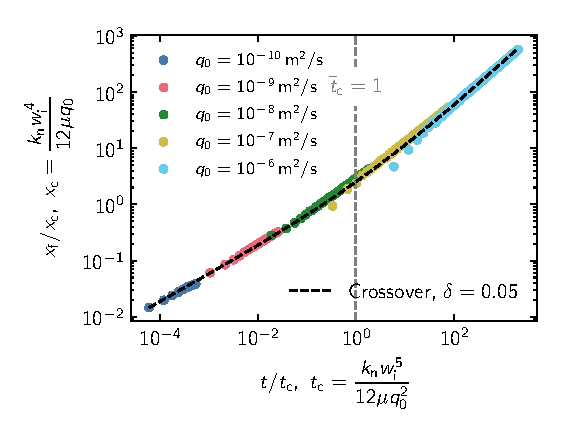
\includegraphics[width=\textwidth]{figures/dimless-front-crossover.eps}
		\end{column}
	\end{columns}
\end{frame}

\begin{frame}
	\frametitle{Fitting crossover function with $\delta=0.05$ produces
		$x_{f}\sim t^{0.7}$ within the timescale of Soultz 1993 seismic sequence}
	\centering
	\vspace{8pt}
	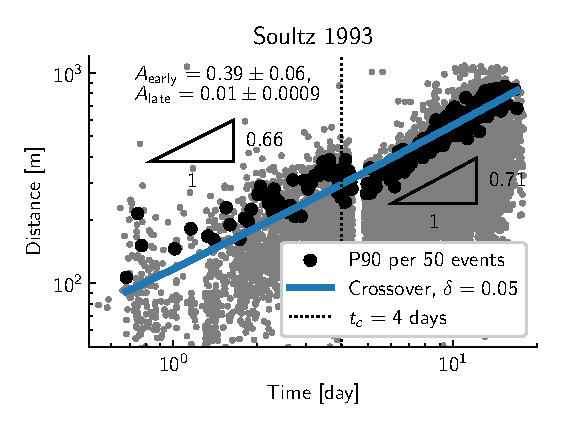
\includegraphics[width=0.6\textwidth]{figures/soultz-crossover.eps}
	$$
		x_{f} = ( 4 D t)^{1/2} = A_{\mathsf{early}} t^{1/2} \to  D=\mathsf{0.03\, m^2/s}
	$$
	$$
		D = \frac{k_{n} w_{i}^{3}}{12 \mu},\, \mathsf{1\, GPa/m} \leq k_{n}
		\leq \mathsf{5000\, GPa/m} \to \mathsf{4.3\, \mu m} \leq w_{i} \leq
		\mathsf{73.0\, \mu m}
	$$
	$$
		x_{f} = a^{1/5} q_{0}^{3/5} t^{4/5} = A_{\mathsf{late}} t^{4/5} \to
		\mathsf{10^{-8}\, m^2/s} \leq q_{0} \leq
		\mathsf{10^{-7}\, m^2/s}
	$$
\end{frame}

\section{Linearly increasing injection rate}


\begin{frame}
	\frametitle{Evolution of dimensionless pressure and front}
    \centering
    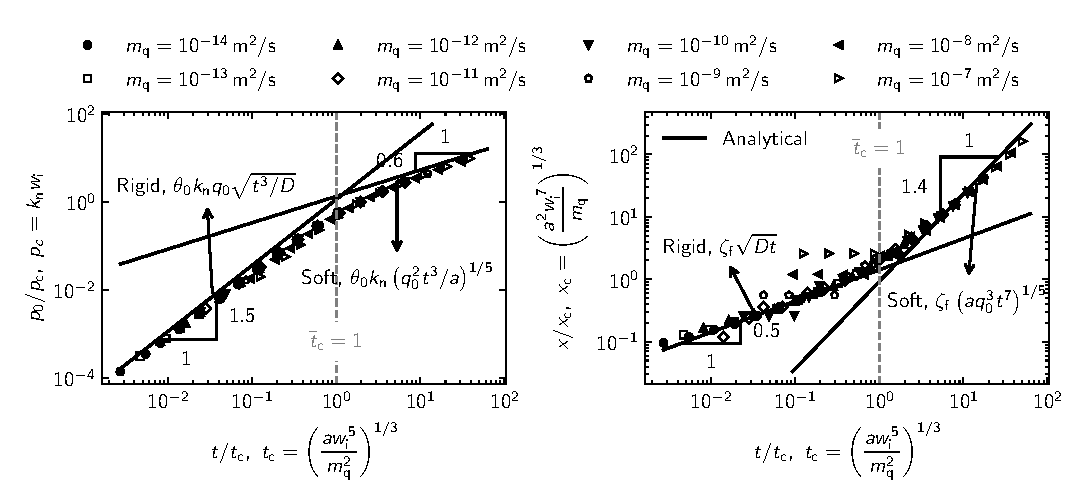
\includegraphics[width=\textwidth]{figures/ramp-inj-dimensionless.eps}

\end{frame}

\end{document}
